\subsection[Verteidigungsgebäude]{Verteidigungsgebäude \hyperref[sec:defence-concept]{\footnotesize $\rightarrow$ Konzept}}
\label{sec:defence}

In Tabelle~\ref{tab:defend-props} werden die Eigenschaften von
Verteidigungsgebäuden beschrieben, Tabelle~\ref{tab:defend-units} enthält die
Gebäude und weist den Eigenschaften Werte zu.

\begingroup
  \small
  \begin{longtabu}{rlX}
    \rowfont{\normalsize}
    \caption{Eigenschaften von Verteidigungsgebäuden\label{tab:defend-props}}\\

    \midrule[\heavyrulewidth]\rowfont{\itshape}
    & Eigenschaft & Beschreibung \\
    \midrule

    K  & Kosten
       & Die Menge an Bitcoin die aufgewendet werden muss, um eines dieser
         Gebäude zu platzieren. \\
    VS & Verteidigungsstärke
       & Schaden, den dieses Gebäude an getroffenen Gegner
         verursacht. \\
    AI & Angriffsintervall
       & Zeit die vergehen muss, bevor dieses Gebäude erneut Gegner angreifen
         kann. \\
    RW & Reichweite
       & Radius um den Turm, in dem Einheiten angegriffen werden können, und in
         dem die Effekte der Türme auf die Einheiten wirken. \\

    \bottomrule
  \end{longtabu}
\endgroup

\begingroup
  \small
  \begin{longtabu}{XXXX}
    \rowfont{\normalsize}
    \caption{Verteidigungsgebäude und ihre Werte\label{tab:defend-units}}
    \\\midrule[\heavyrulewidth]\endfirsthead

    \rowfont{\normalsize}
    \caption[]{Verteidigungsgebäude und ihre Werte (fortges.)}
    \\\midrule[\heavyrulewidth]\endhead

    \multicolumn{4}{r}{\itshape fortges. auf der nächsten Seite}
    \\\endfoot

    \endlastfoot

    \multicolumn{4}{c}{\bfseries Kabel} \\*
    K: 10 & VS: -- & AI: -- & RW: -- \\\midrule
    \multicolumn{4}{p{\bodywidth}}{%
      \begin{minipage}{0.85\linewidth}
        Dieses Gebäude kostet wenig, steht gegnerischen Einheiten im Weg und
        verursacht keinen Schaden.
      \end{minipage}\hfill\parbox{0.15\linewidth}{%
        \hfill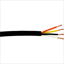
\includegraphics[scale=0.5]{verteidigung/wires.png}\hfill\null}}
    \\\bottomrule

    \multicolumn{4}{c}{\bfseries Mauszeigerschütze} \\*
    K: 20 & VS: 2  & AI: 1  & RW: 6  \\\midrule
    \multicolumn{4}{p{\bodywidth}}{%
      \begin{minipage}{0.85\linewidth}
        Durchschnittlicher Verteidigungsturm, der Mauszeiger auf ein Einzelziel
        verschießt.
      \end{minipage}\hfill\parbox{0.15\linewidth}{%
        \hfill
\includegraphics[scale=0.5]{verteidigung/mouse.png}\hfill\null}}
    \\\bottomrule

    \multicolumn{4}{c}{\bfseries CD-Werfer} \\*
    K: 20 & VS: 5  & AI: 2  & RW: 4  \\\midrule
    \multicolumn{4}{p{\bodywidth}}{%
      \begin{minipage}{0.85\linewidth}
        Dieser Turm kostet mehr und schießt langsamer als ein
        \emph{Mauszeigerschütze,} dafür verursacht das Projektil (die CD)
        jedoch auf ihrem Weg an jedem berührten Gegner den Schaden der Höhe VS.
      \end{minipage}\hfill\parbox{0.15\linewidth}{%
        \hfill
\includegraphics[scale=0.6]{verteidigung/cd_thrower.png}\hfill\null}}
    \\\bottomrule

    \multicolumn{4}{c}{\bfseries Antivirusprogramm} \\*
    K: 30 & VS: 8  & AI: 3  & RW: 10 \\\midrule
    \multicolumn{4}{p{\bodywidth}}{%
      \begin{minipage}{0.85\linewidth}
        Von den Kosten ist dieser Turm vergleichbar zum \emph{CD-Werfer,}
        allerdings schießt das \emph{Antivirusprogramm} noch langsamer,
        verursacht dafür aber an einem Einzelziel erheblichen Schaden.
      \end{minipage}\hfill\parbox{0.15\linewidth}{%
        \hfill
\includegraphics[scale=0.6]{verteidigung/antivirus.png}\hfill\null}}
    \\\bottomrule

    \multicolumn{4}{c}{\bfseries Lüftung} \\*
    K: 20 & VS: 0  & AI: -- & RW: 3  \\\midrule
    \multicolumn{4}{p{\bodywidth}}{%
      \begin{minipage}{0.85\linewidth}
        Dieser Turm verlangsamt alle Einheiten im Einflussbereich. Der Turm hat
        keine Abklingzeit.
      \end{minipage}\hfill\parbox{0.15\linewidth}{%
        \hfill
\includegraphics[scale=0.6]{verteidigung/fan.png}\hfill\null}}
    \\\bottomrule

    \multicolumn{4}{c}{\bfseries Wifi-Router} \\*
    K: 40 & VS: 1  & AI: 1  & RW: 2  \\\midrule
    \multicolumn{4}{p{\bodywidth}}{%
      \begin{minipage}{0.85\linewidth}
        Dieser Turm schießt nahezu dauerhaft kreisförmige Wellen, die wenig
        Schaden verursachen und Gegner penetrieren.
      \end{minipage}\hfill\parbox{0.15\linewidth}{%
        \hfill
\includegraphics[scale=0.6]{verteidigung/router.png}\hfill\null}}
    \\\bottomrule

    \multicolumn{4}{c}{\bfseries Schockfeld} \\*
    K: 40 & VS: 2  & AI: 3  & RW: -- \\\midrule
    \multicolumn{4}{p{\bodywidth}}{%
      \begin{minipage}{0.85\linewidth}
        Dieser „Turm“ blockiert die Gegner nicht, sie laufen darüber hinweg.
        In regelmäßigen Abständen erhalten alle Gegner schaden, die auf einem
        \emph{Schockfeld} sind.
      \end{minipage}\hfill\parbox{0.15\linewidth}{%
        \hfill
\includegraphics[scale=0.6]{verteidigung/shock_field.png}\hfill\null}}
    \\\bottomrule
  \end{longtabu}
  \missingpics{Bilder für Verteidigungsgebäuden}
\endgroup
